\textbf{B.4: HC-05 Bluetooth Modül}
\label{YedinciBolum}

	HC-05 Bluetooth modülü,  kablosuz seri haberleşme projeleri için yapılmıştır. Bu modül bluetooth 2.0’ı destekleyen, 2.4GHz frekansında haberleşme yapılmasını sağlar. Haberleşme esnasında açık alanda yaklaşık 10 metre haberleşme mesafesine sahiptir. Modülün haberleşme bağlantısı serial yani UART olduğundan kolay ve hızlı bir kullanımı vardır. Üzerinde bulunan RX ve TX pinleri sayesinde iletişim sağlanır. Bu pinler kullanılacak olan devre kartınının sırasıyla TX ve RX pinlerine bağlanır. Ayrıca bu pinler yardımıyla AT komutlarını kullanarak modülün isim, şifre,baud rate değeri, gibi çeşitli özellikleri değiştirebilir. KAYNAK [3]
    
	Projede ise bu modül kablosuz haberleşme için kullanılmaktadır. Bilgisayar veya mobil üzerinden alınan analog veriler bu modül sayesinde tarete aktarılmaktadır. Bu sayede kullanıcı tarafından yapılan hareketleri anlık olarak taret üzerinde de gözlemleyebiliriz. Bluetooth modül Şekil 7de gösterilmiştir.

\begin{figure}[H]
	\centering
	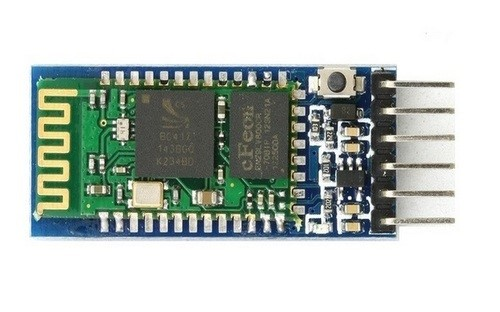
\includegraphics[width=100mm]{grafik/Bluetooth.jpg}
    \caption{Projede Kullanılan HC-05 Bluetooth Modülü}
	\label{fig:BluetoothDM}
\end{figure}

\textbf{Dikkat:} HC-05 Bluetooth modülü devre kartındaki 3.3V pinine bağlantı yapılarak veya uçları arasında dirençler bağlayarak çalıştırılması gerekmektedir. HC-06 Bluetooth modülü ise 5V pinine bağlantı yapılarak veya yine direnç bağlanarak çalıştırılmalıdır.

\textbf{Bilgi:} Kodları hatasız bir şekilde Arduino’ya aktarabilmek için Arduino üzerindeki RX ve TX pinlerine bağlı kabloları aktarma işleminden önce sökmek gerekiyor. Bu işlem yapılmazsa kod aktarımı sırasında portların meşgul olduğuna dair hata alabiliriz. 

\clearpage